%%%%%%%%%%%%%%%%%%%%%%%%%%%%%%%%%%%%%%%%%
% Beamer Presentation
% LaTeX Template
% Version 1.0 (10/11/12)
%
% This template has been downloaded from:
% http://www.LaTeXTemplates.com
%
% License:
% CC BY-NC-SA 3.0 (http://creativecommons.org/licenses/by-nc-sa/3.0/)
%
%%%%%%%%%%%%%%%%%%%%%%%%%%%%%%%%%%%%%%%%%

%----------------------------------------------------------------------------------------
%	PACKAGES AND THEMES
%----------------------------------------------------------------------------------------

\documentclass{beamer}

\mode<presentation> {

% The Beamer class comes with a number of default slide themes
% which change the colors and layouts of slides. Below this is a list
% of all the themes, uncomment each in turn to see what they look like.

%\usetheme{default}
%\usetheme{AnnArbor}
%\usetheme{Antibes}
%\usetheme{Bergen}
%\usetheme{Berkeley}
%\usetheme{Berlin}
%\usetheme{Boadilla}
%\usetheme{CambridgeUS}
%\usetheme{Copenhagen}
%\usetheme{Darmstadt}
%\usetheme{Dresden}
%\usetheme{Frankfurt}
%\usetheme{Goettingen}
%\usetheme{Hannover}
%\usetheme{Ilmenau}
%\usetheme{JuanLesPins}
%\usetheme{Luebeck}
\usetheme{Madrid}
%\usetheme{Malmoe}
%\usetheme{Marburg}
%\usetheme{Montpellier}
%\usetheme{PaloAlto}
%\usetheme{Pittsburgh}
%\usetheme{Rochester}
%\usetheme{Singapore}
%\usetheme{Szeged}
%\usetheme{Warsaw}

% As well as themes, the Beamer class has a number of color themes
% for any slide theme. Uncomment each of these in turn to see how it
% changes the colors of your current slide theme.

%\usecolortheme{albatross}
%\usecolortheme{beaver}
%\usecolortheme{beetle}
%\usecolortheme{crane}
%\usecolortheme{dolphin}
%\usecolortheme{dove}
%\usecolortheme{fly}
%\usecolortheme{lily}
%\usecolortheme{orchid}
%\usecolortheme{rose}
%\usecolortheme{seagull}
%\usecolortheme{seahorse}
%\usecolortheme{whale}
%\usecolortheme{wolverine}

%\setbeamertemplate{footline} % To remove the footer line in all slides uncomment this line
%\setbeamertemplate{footline}[page number] % To replace the footer line in all slides with a simple slide count uncomment this line

%\setbeamertemplate{navigation symbols}{} % To remove the navigation symbols from the bottom of all slides uncomment this line
}

\usepackage{graphicx} % Allows including images
\usepackage{booktabs} % Allows the use of \toprule, \midrule and \bottomrule in tables
\usepackage{listings}

\lstdefinestyle{customjava}{
  breaklines=true,
  frame=L,
  xleftmargin=\parindent,
  language=Java,
  showstringspaces=false,
  basicstyle=\footnotesize\ttfamily,
  keywordstyle=\bfseries\color{green!40!black},
  commentstyle=\itshape\color{gray!40!black},
  identifierstyle=\color{blue},
  stringstyle=\color{orange},
}
%----------------------------------------------------------------------------------------
%	TITLE PAGE
%----------------------------------------------------------------------------------------

\title[Java Generics]{Java Generics } % The short title appears at the bottom of every slide, the full title is only on the title page

\author{Jonathan Windle} % Your name
\institute[UEA] % Your institution as it will appear on the bottom of every slide, may be shorthand to save space
{
University of East Anglia \\ % Your institution for the title page
\medskip
\textit{J.Windle@uea.ac.uk} % Your email address
}
\date{\today} % Date, can be changed to a custom date

\begin{document}

\begin{frame}
\titlepage % Print the title page as the first slide
\end{frame}

\begin{frame}[allowframebreaks]
\frametitle{Overview} % Table of contents slide, comment this block out to remove it
\tableofcontents % Throughout your presentation, if you choose to use \section{} and \subsection{} commands, these will automatically be printed on this slide as an overview of your presentation
\end{frame}

%----------------------------------------------------------------------------------------
%	PRESENTATION SLIDES
%----------------------------------------------------------------------------------------

%------------------------------------------------
\section{Using Generics} % Sections can be created in order to organize your presentation into discrete blocks, all sections and subsections are automatically printed in the table of contents as an overview of the talk
%------------------------------------------------

\subsection{Typing Data Structures/Raw Types} % A subsection can be created just before a set of slides with a common theme to further break down your presentation into chunks
\defverbatim[colored]\arr{
\begin{lstlisting}[style = customjava,basicstyle=\ttfamily]
ArrayList arr = new ArrayList();
\end{lstlisting}
}

\defverbatim[colored]\arrTwo{
\begin{lstlisting}[style = customjava,basicstyle=\ttfamily]
arr.add("Boop");
arr.add(8004);
String str = (String) arr.get(0);
\end{lstlisting}
}
\begin{frame}
\frametitle{Typing Data Structures/Raw Types}
\arr
\begin{itemize}
\item By default \texttt{ArrayList} is designed to store Object references.
\item This means anything can be added except primitive types.
\item \texttt{ArrayList} is \textbf{completely generic} in that it can store anything. It is said to be a {\color{red} Raw Type}.
\end{itemize}
\arrTwo
\begin{itemize}
\item \texttt{arr} is {\color{red} raw type}, when getting something from the \texttt{arr} it is necessary to cast as get returns \texttt{Object}
\end{itemize}
\end{frame}

%------------------------------------------------
\subsection{Issues With Raw Types}
\begin{frame}
\frametitle{Issues with Raw Types}
\begin{itemize}
\item Completely dependant on the user to correctly use structure.
\item If the user misuses the casting and cast the wrong type, an Exception will be thrown. This is detected at {\color{red} run time}.
\end{itemize}
\end{frame}
%------------------------------------------------
\subsection{Generics}
\begin{frame}
\frametitle{Generics}
\begin{itemize}
\item Enforces a data structure to only contains \texttt{Objects} of a certain type using Generic syntax.
\item Removes the need for casting, ensuring {\color{green} type safety}.
\item Any potential casting errors are detected at {\color{red} Compile time}.
\item \texttt{<>} Diamond operator means type is ensured from the left hand side of the assignment, not the same as assigning a {\color{purple} raw type}.
\item Interfaces are commonly Generic, such as {\color{blue} Comparable} and {\color{orange} Comparator}. This means there is no need to cast and interfaces can be used freely.
\end{itemize}
\end{frame}
%-------------------------------------------------
\subsection{Basics Summary}
\begin{frame}
\frametitle{Basics Summary}
\begin{itemize}
\item Means of enforcing {\color{green} type safety} on data structures without defining multiple classes for each type.
\item Allow for early {\color{orange} error detection at compile time}.
\item Removes need for casting.
\end{itemize}
\end{frame}
%------------------------------------------------
\section{How Generics Work}
\subsection{Compiling Generic Code}
\begin{frame}
\frametitle{Compiling Generic Code}
\begin{itemize}
\item Two possible strategies:
\begin{itemize}
\item Create a new class for every different type used ({\color{red} code specialisation}) - {\color{orange} C++ not Java}.
\item Use one general class and determine types at runtime ({\color{green} code sharing}).
\end{itemize}
\end{itemize}
\end{frame}
%------------------------------------------------
\subsection{Code Specialisation - C++}
\begin{frame}
\frametitle{Code Specialisation - C++}
\begin{itemize}
\item Compiler generates a new representation for every instantiation of a generic type or method
\item At compile time:
\begin{enumerate}
\item Form a list of all types of the data structure defined in the code.
\item Create a new class of that data structure and compile seperately.
\end{enumerate}
\item {\color{green} Benefits:}
\begin{itemize}
\item No impact on runtime performance.
\item Easy to optimize compilation.
\end{itemize}
\item {\color{red} Problems:}
\begin{itemize}
\item You need to know at compile time all possible types.
\end{itemize}
\end{itemize}
\end{frame}
%-------------------------------------------------
\subsection{Code Sharing: Type Erasure - Java}
\begin{frame}
\frametitle{Code Sharing: Type Erasure - Java}
\begin{itemize}
\item Compiler generates code for only one representation of a generic type, by {\color{orange}erasing} the Generic type and replacing with \texttt{Object}.
\item At compile time:
\begin{enumerate}
\item All types are stripped from a generic and compiled as a {\color{purple} raw type}.
\item {\color{magenta}Type checks and casts} are automatically added. These are performed at runtime.
\end{enumerate}
\item {\color{green} Benefit:}
\begin{itemize}
\item No need to create extra files which may not be needed.
\end{itemize}
\item {\color{red} Problem: }
\begin{itemize}
\item Extra type checking takes time, slower execution.
\end{itemize}
\end{itemize}
\end{frame}
%-------------------------------------------------------
\section{Writing Generic Classes}
\subsection{Simple Generic Data Structures}
\begin{frame}
\frametitle{Simple Generic Data Structures}
\begin{itemize}
\item \texttt{<E> E} represents the {\color{red} enforced} type chosen.
\item Can still instantiate a {\color{orange} raw type} of any generic.
\item \texttt{<K,V,E,S>} You can have as many types as you want and use any valid identifier.
\end{itemize}
\end{frame}
%--------------------------------------------------------
\subsection{Generics in nested classes}
\defverbatim[colored]\genNest{
\begin{lstlisting}[style = customjava,basicstyle=\scriptsize]
public class Pair<K,V> {
	public class Inner {
    	K in1; // K is same type as outer class 
        V in2; // V is same type as outer class
    }
}
\end{lstlisting}
}
\defverbatim[colored]\genNestTwo{
\begin{lstlisting}[style = customjava,basicstyle=\scriptsize]
public class Pair<K,V> {
	public static class Inner {
    // Cannot reference either K or V due to static instance
    }
	public static class Inner<K,V> {
    // Type can be set independently to the outer object
    	K in1; // K is same label, could be different Type
        V in2; // V is same label, could be different Type
    }
}
\end{lstlisting}
}
\begin{frame}
\frametitle{Generics in nested classes}
\begin{itemize}
\item {\color{orange}Nested classes} can have the same generic type as outer class, due to always being associated with an instance of the outer class.
\genNest
\item {\color{purple} Static nested classes} \textbf{cannot} refer to generic type of enclosing class.
\genNestTwo
\end{itemize}
\end{frame}
%--------------------------------------------------------
\defverbatim[colored]\genCom{
\begin{lstlisting}[style = customjava,basicstyle=\tiny]
public class Pair<K,V> implements Comparable<K,V>> {
	private K key;
    private V value;
    public int compareTo(Pair<K,V> other) {
    	return key.compareTo(other.key); // NOT ALLOWED Key not necessarily comparable
    }
}
\end{lstlisting}
}
\defverbatim[colored]\genComTwo{
\begin{lstlisting}[style = customjava,basicstyle=\tiny]
public class Pair<K,V> implements Comparable<K extends Comparable,V>> {
	private K key;
    private V value;
    public int compareTo(Pair<K,V> other) {
    	return key.compareTo(other.key); // K Has to be Comparable, this is allowed
    }
}
\end{lstlisting}
}
\subsection{Enforcing Generic Restrictions}
\begin{frame}
\frametitle{Enforcing Generic Restrictions}
\begin{itemize}
\item The type of a generic can be typed using the {\color{red} extends} keyword. \item \texttt{<T {\color{blue}extends} Number>} Means you can only type the generic to \texttt{Number} or a subclass of \texttt{Number}.
\item Making generics comparable:
\item {\color{red} NOT ALLOWED} - without enforcing restriction
\genCom
\item {\color{green} ALLOWED:} - with enforcing using \texttt{{\color{blue} extends} Comparable}
\genComTwo
\end{itemize}
\end{frame}
%--------------------------------------------------------
\begin{frame}
\frametitle{Enforcing Generic Restrictions - Cont.}
\begin{itemize}
\item {\color{red} Type Erasure} replaces the generic type with the least specific restriction.
\item If requirement is several interfaces, they can be enforced by \& e.g. \texttt{<T {\color{blue} extends} Comparable<T> \& Cloneable>}
\end{itemize}
\end{frame}
%--------------------------------------------------------
\defverbatim[colored]\genMeth{
\begin{lstlisting}[style = customjava,basicstyle=\ttfamily]
String[] sa = new String[10];
insertionSort(sa); // Infers String type

Integer[] in = new Integer[50];
insertionSort(in); // Infers integer type
\end{lstlisting}
}
\subsection{Generic Methods}
\begin{frame}
\frametitle{Generic Methods}
\begin{itemize}
\item Work in a very similar way to classes. Type scope is limited to that method only though.
\item Don't have to explicitly pass the type arguments, it's inferred from arguments passed.
\item \texttt{insertionSort()} is a generic method:
\genMeth
\end{itemize}
\end{frame}
%--------------------------------------------------------
\subsection{Wildcards}
\begin{frame}
\frametitle{Wildcards}
\begin{itemize}
\item Three types of wildcard:
\begin{itemize}
\item ?: denotes {\color{red} set of all types}
\item ? {\color{blue} extends Foo} Denotes a {\color{green}family of subtypes of type Foo}
\item ? {\color{blue} super Bar} Denotes a {\color{purple}family of supertypes of type Bar}
\end{itemize}
\item The main use of wildcards is to overcome the problem with {\color{orange} inheritance} and generics.
\end{itemize}
\end{frame}
%--------------------------------------------------------
\defverbatim[colored]\wild{
\begin{lstlisting}[style = customjava,basicstyle=\tiny]
Wrapper<?> raw; // Unbounded, any type.
Wrapper<? super Number> up; // Number or any superclass
Wrapper<? extends Number> down; // Number or any subclass 
up = new Wrapper<Object>(); // This is OK
down = new Wrapper<Double>(); // This is also OK.
\end{lstlisting}
}
\begin{frame}
\frametitle{Wildcards - Cont.}
\wild
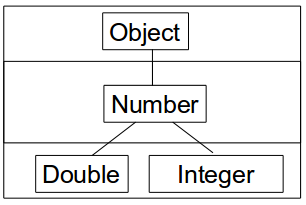
\includegraphics[scale=0.5]{wildcards.png}
\begin{itemize}
\item In this case, up can be in the top half or Number.
\item down can be anything in the middle or lower half.
\end{itemize}
\end{frame}
%--------------------------------------------------------
\defverbatim[colored]\wildAll{
\begin{lstlisting}[style = customjava,basicstyle=\tiny]
LinkedList<Number> m2 = new LinkedList<>();
m2.add(new Integer(11)); // Is allowed
m2.add(new Double(2.5)); // Is allowed
\end{lstlisting}
}
\defverbatim[colored]\wildNot{
\begin{lstlisting}[style = customjava,basicstyle=\tiny]
LinkedList<Number> m = new LinkedList<Integer>(); // Not allowed
LinkedList<Number> m = new LinkedList<Double>(); // Not allowed
\end{lstlisting}
}
\subsection{Why we need wildcards}
\begin{frame}
\frametitle{Why we need wildcards}
\begin{itemize}
\item There is no inheritance between generics of different types.
\item You can store subclasses in in a typed structure e.g.:
\wildAll
\item You cannot store generic subclasses e.g.:
\wildNot
\item \texttt{LinkedList<Number>} is not a {\color{red} superclass} of \texttt{LinkedList<Double>}.
\item {\color{green} Type erasure} does not allow for this. Generic collections are {\color{orange} invariant}
\end{itemize}
\end{frame}

%--------------------------------------------------------
\defverbatim[colored]\wildUse{
\begin{lstlisting}[style = customjava,basicstyle=\tiny]
// This can only be used for Object arrays.
static void printList(ArrayList<Object> list) {
	for (Object elem : list) {
		System.out.println(elem);
	}
}
ArrayList<String> strArr = new ArrayList<>();
strArr.add("Boop");
printList(strArr); // This won't compile. 

\end{lstlisting}
}

\defverbatim[colored]\wildUseTwo{
\begin{lstlisting}[style = customjava,basicstyle=\tiny]
// This can be used with ANY ArrayList
static void printList(ArrayList<?> list) {
	for (Object elem : list) {
		System.out.println(elem);
	}
}
ArrayList<String> strArr = new ArrayList<>();
ArrayList<Card> cardArr = new ArrayList<>();
printList(strArr); // This is OK
printList(cardArr); // This is OK
\end{lstlisting}
}
\subsection{Wildcard use case}
\begin{frame}
\frametitle{Wildcard use case}
\begin{itemize}
\item This will not work due to no inheritance between generics.
\item \texttt{ArrayList<String>} is {\color{red} not} the same as \texttt{ArrayList<Object>}
\wildUse
\item With the use of {\color{green} wildcard ?} this will work with any \texttt{ArrayList} and keep {\color{purple} Type safety}
\wildUseTwo
\end{itemize}
\end{frame}
%--------------------------------------------------------
\subsection{Random Generic things}
\begin{frame}
\frametitle{Generic Arrays don't work}
\begin{itemize}
\item Array's have a dynamic type, i.e. \texttt{Object[]} can store \texttt{Integer} references, but {\color{red} type erasure} does not use it.
\item Solution is to cast Generic arrays to \texttt{Object[]} or use \texttt{ArrayList}.
\end{itemize}
\end{frame}
%--------------------------------------------------------
\section{Summary}
\begin{frame}
\frametitle{Summary}
\begin{itemize}
\item Generics are a way of enforcing a type on a data structure.
\item Errors can be found at {\color{green} compile time}
\item Restrictions at {\color{purple} Class level} can be put in place using \texttt{\color{blue} extends}.
\item Restrictions on a type can be removed at the {\color{orange} Object level} using \texttt{\color{red} wildcards}.
\end{itemize}
\end{frame}
%--------------------------------------------------------
\subsection{What we should know...?}
\begin{frame}
\frametitle{What we should know...?}
\begin{itemize}
\item Benefits of generics
\item Differences between {\color{green} code sharing (Type Erasure)} and {\color{red}Code specialisation} and which language does what.
\item Understanding of restrictions that can be put on.
\item Methods can be generic so they can be used with generic classes.
\end{itemize}
\end{frame}
%--------------------------------------------------------
\begin{frame}
\Huge{\centerline{The End}}
\end{frame}

%----------------------------------------------------------------------------------------

\end{document}